%!TEX root = ../../../adrien_gomar_phd.tex

The HB method has been originally
proposed by \citet{Hall2002}, at that time named
Harmonic Balance Technique (HBT).
It can be considered as an improvement of the NLFD
approach. In fact, instead
of using the fast Fourier transform to cast back the equations
to the time domain at each pseudo-iteration step, 
the equations are mathematically derived to be directly
computed into the time-domain.
To explain the method, we will again use the general form of 
the non-viscous Burger's equation as defined in
Eq.~\eqref{eq:sm_nonlinear_convection_residual}.
This thesis rely on the former work of \citet{ThesisSicot} who
implemented the harmonic balance method into the 
\textit{elsA}~\cite{Cambier2013} CFD code at CERFACS. 
Recently \citet{ThesisGuedeney} extended it to the
multi-frequential formulation, allowing contra-rotating
open rotor aeroelastic computations. This is why this
approach will be used in the current work.

\subsection{Mono-frequential formulation}

Following the same approach as the non-linear frequency domain one,
it is considered that both $u$ and $R$ are periodic
in time with respect to period $T = 2 \pi / \omega$
and can be written using Fourier series:
\begin{equation}
	\begin{split}
		u(t) &= \sum_{k=-\infty}^{\infty} \widehat{u}_k e^{i k \omega t}, \\
		R(t) &= \sum_{k=-\infty}^{\infty} \widehat{R}_k e^{i k \omega t}.
		\label{eq:sm_hall_dft}
	\end{split}
\end{equation}
Injecting Eq.~\eqref{eq:sm_hall_dft} in 
Eq.~\eqref{eq:sm_nonlinear_convection_residual}, and considering
the orthogonality of the complex exponentials:
\begin{equation}
	i k \omega \widehat{u}_k + \widehat{R}_k = 0, \: k \in [-N, N].
	\label{eq:sm_hall_frequential_eq}
\end{equation}

In the same way as one uses Fourier coefficients to
evaluate the temporal signal,
one can reconstruct the Fourier coefficients using
temporal evaluations. These are taken at evenly spaced time instances
sampling the period $T = 2 \pi / \omega$. Moreover, 
according to the Nyquist-Shannon~\cite{Shannon1949} sampling theorem, 
at least $2N$ time instances are needed to capture $N$ frequencies. Actually
$2N+1$ time instances are used to prevent odd-even decoupling as
demonstrated by \citet{Weide2005}. $\widehat{u}_k$ can thus
be expressed in function of $u(t)$ using the inverse
Fourier transform:
\begin{equation}
	\widehat{u}_k = \frac{1}{2N+1} 
	\sum_{n=0}^{2N} u(t_n) e^{-i k \omega t_n}.
\end{equation}
If $E$ denotes the matrix composed of the elements 
$(E)_{k,n} = e^{-i (k - N) \omega t_n} / 2N+1$, one can write $\widehat{u}_k$
and $\widehat{R}_k$ as:
\begin{equation}
	\begin{split}
		\widehat{u}_k &= E u^\star, \\
		\widehat{R}_k &= E R^\star,
	\end{split}
	\label{eq:sm_matrix_fourier_operator}
\end{equation}
where $u^\star$ and $R^\star$ 
denote the vectors formed of all the evaluations of $u$
and $R$, respectively,
made at $2N+1$ time instances uniformly sampling the period of interest:
\begin{equation}
	\begin{split}
		u^\star &= [u(t_0) \cdots u(t_{2N})], \\
		R^\star &= [R(t_0) \cdots R(t_{2N})].
	\end{split}
\end{equation}
$E$ can thus be named the Fourier matrix.
Note that conversely, using the inverse Fourier matrix $E^{-1}$:
\begin{equation}
	\begin{split}
		u^\star &= E^{-1} \widehat{u}_k \\
		R^\star &= E^{-1} \widehat{R}_k.
	\end{split}
	\label{eq:sm_sampling_hb_var}
\end{equation}
Injecting the matrix formulation of 
Eq.~\eqref{eq:sm_matrix_fourier_operator} in 
Eq.~\eqref{eq:sm_hall_frequential_eq}
gives:
\begin{equation}
	i \omega K E u^\star + E R^\star = 0,
\end{equation}
where $K$ is a diagonal matrix formed of all the $k \in [-N, N]$.
Note that first, the matrix formulation encompass all harmonics
$k \in [-N, N]$ and second, it does not require the
orthogonality of the complex exponentials.
Now multiplying the equation by the inverse Fourier matrix $E^{-1}$:
\begin{equation}
	i \omega E^{-1} K E u^\star + R^\star = 0,
	\label{eq:sm_hb_matrix_form_mono}
\end{equation}
where $R^\star$ can now be substituted:
\begin{equation}
		i \omega E^{-1} K E u^\star + 
		\displaystyle \frac{\partial}{\partial x}
		\frac{(u^\star)^2}{2} = 0.
\end{equation}
What happened here is that instead of developing $R(t)$
in the frequency domain as made with the NLH approach,
which is tedious, this term is kept
in this form through all the development process. 
Since $R(t)$ only includes spatial derivatives, no temporal non-linear
terms
arise by using the Fourier decomposition. Thus, multiplying it
by the inverse Fourier matrix leads to the unity matrix. 
$R(t)$ is then simply evaluated at $2N+1$ time instances.

This approach is really close to the NLFD method.
The higher order perturbation terms are taken into account
in the equations.
% The reader might observe that we are introducing the discrete Fourier
% transform and its inverse. This is close to the fast Fourier transform
% and its inverse, as proposed by \citet{McMullen2001}. 
However,
as the development is on the equations and not during the time loop,
we get $2N+1$ steady equations, by definition in the time
domain, that are coupled by a source term.
The source term appears as a spectral operator defined as:
\begin{equation}
	D_t = i \omega E^{-1} K E.
	\label{eq:sm_hb_mono_source_term_matrix}
\end{equation}

To compute $D_t$, \citet{Hall2002}
inverse the Fourier matrix $E$.
In an easier way, \citet{Gopinath2005} provided 
an analytical formulation of the source term defined 
in Eq.~\eqref{eq:sm_hb_mono_source_term_matrix} and 
named the HB approach the Time Spectral Method (TSM).
It is a matrix operator whose elements are defined as:
\begin{equation}
  (D_t)_{k, n} =
  \begin{cases}
    \frac{\pi}{T}(-1)^{k-n}\csc\left(\frac{\pi
        (k-n)}{2N+1}\right) &, \, k\neq n,\\
    0 &, \, k=n.
  \end{cases}
  \label{eq:sm_hb_mono_source_term_analytic}
\end{equation}
The main difference with the NLFD approach
is that the source term matrix $D_t$ is known at the first iteration and does
not change, meaning that we do not spend time computing a
fast Fourier transform and its inverse at each time-step.
Finally, adding a pseudo-time ($\tau$) derivative to 
time march the equations to the steady state, 
the mono-frequential formulation of 
Eq.~\eqref{eq:sm_nonlinear_convection_conservative} in the harmonic
balance framework is given by:
\begin{equation}
	\fbox{$
	\displaystyle \frac{\partial u^\star}{\partial \tau} + 
	D_t (u^\star) + 
	\displaystyle \frac{\partial}{\partial x}
		\frac{(u^\star)^2}{2} = 0
	$}
\end{equation}
with $D_t$ defined using Eq.~\eqref{eq:sm_hb_mono_source_term_analytic}.
As for the NLFD method, the term $u^\prime u^\prime$
is not neglected in the current approach.

\subsection{Multi-frequential formulation}
\label{sec:sm_hb_multi}
In the
framework of almost-periodic functions~\cite{Besicovitch1932},
such a function $f(t)$ (which is composed of multiple
frequencies non necessarily harmonically related) can be approximated
by an almost-periodic
discrete Fourier transform:
\begin{equation}
	f(t) \approx \sum_{k=-N}^{N} \widehat{f}_k 
	e^{i \omega_k t}.
\end{equation}
In this framework, \citet{Gopinath2007} and \citet{Ekici2007} 
extended the harmonic balance approach to
a multi-frequential formulation. To do so, they considered
a Fourier matrix defined as:
\begin{equation}
	(E)_{k,n} = \frac{1}{2N+1} e^{-i \omega_{k-N} t_n},
\end{equation}
where $N$ is the chosen number of frequencies.
Note that replacing $\omega_{k-N}$ by $(k - N) \omega$ gives
the mono-frequential inverse Fourier matrix back. 
However, in the multi-frequential case, the inverse Fourier matrix
$E^{-1}$ has to be numerically computed from $E$. Actually, as demonstrated by 
\citet{Gopinath2007}, it is easier to express $E^{-1}$ analytically,
compute its temporal derivative (that is hence analytical too) 
and inverse it numerically to obtain $E$. In fact, the source term
can be written as $D_t = \frac{\partial E^{-1}}{\partial t} E$
which ease its computation.

Using the same process as for the mono-frequential formulation,
Eq.~\eqref{eq:sm_nonlinear_convection_residual} becomes:
\begin{equation}
	i E^{-1} P E u^\star + R^\star = 0,
\end{equation}
where $P$ is a diagonal matrix formed of all the angular frequencies $\omega_k$.
Note that the exponentials do not need to form an
orthogonal family here. The only need is to have the multi-frequential
Fourier matrix $E$ to be invertible which is the case~\cite{Ekici2007}.
This is really close to the mono-frequential formulation given
in Eq.~\eqref{eq:sm_hb_matrix_form_mono}.
Finally, adding a pseudo-time ($\tau$) derivative 
to time-march the equations to the steady state,
the multi-frequential formulation of 
Eq.~\eqref{eq:sm_nonlinear_convection_conservative} in the harmonic
balance framework reads:
\begin{equation}
	\fbox{$
	\displaystyle \frac{\partial u^\star}{\partial \tau} +
	D_t (u^\star) + 
	\displaystyle \frac{\partial}{\partial x}
		\frac{(u^\star)^2}{2} = 0
	$}
\end{equation}
with $D_t$ defined as:
\begin{equation}
	D_t = i E^{-1} P E,
	\label{eq:sm_multi_spectral_operator}
\end{equation}
and again $u^\star = [u(t_0) \cdots u(t_{2N})]$ 
and $R^\star = [R(t_0) \cdots R(t_{2N})]$.

\subsection{Extensions}
\label{sec:sm_hb_extension}

\paragraph{Navier--Stokes equations}
As for the NLFD approach, since the 
Navier--Stokes equations can be written in finite-volume,
semi-discrete form as:
\begin{equation}
	V \frac{\partial W}{\partial t} + R(W) = 0,
\end{equation}
nothing particular has to be made to derive this approach for
the Navier--Stokes equations, except adding the source term computation
in the time-loop.
This shows its advantage over the NLFD and particularly over the NLH method.

\paragraph{Turbomachinery computations}
Originally, the HB method has been developed for 
turbomachinery applications.
\citet{Hall2002} applied the method to the computation
of the flutter boundary of the front stage rotor 
of a modern high-pressure transonic compressor. To reduce the
computational domain to a single blade passage, 
a phase-lagged boundary condition is used at the azimuthal
interfaces:
\begin{equation}
	\widehat{u}_{k, U} = \widehat{u}_{k, L} e^{i \sigma k},
\end{equation}
for $k \in [-N, N]$, where subscript $U$ and $L$ denote
respectively the upper and lower azimuthal boundaries, and
$\sigma$ denotes the inter-blade phase angle. This boundary
condition allows to compute isolated aeroelastic configurations
using only one blade-passage.
\Citet{Weide2005} extended the approach to take into account
for the periodic boundary conditions when the equations are solved in the
cartesian coordinate system. The efficiency of the
method was demonstrated with the NASA-Stage~$35$ compressor. In that case,
engineering accuracy is obtained with only $N=5$ harmonics.
Nothing is said on the strategy used at the rows interface.

\citet{Ekici2007} and \citet{Gopinath2007}
extended the method to a multi-frequential formulation. 
As such, it can then be applied to multi-stage
configurations. Both of them demonstrated the application of
the method on
a two-dimensional multi-stage compressor called
configuration~D. 
The strategy used by \citet{Ekici2007} 
to exchange the variables at
the rows interface is schematically represented 
in Fig.~\ref{fig:bnd_sliding_ekici2007}.
\begin{figure}[htp]
  \centering
  \includegraphics*[scale=0.25]{bnd_sliding_ekici2007.pdf}
  \caption{Exchange of the variable at rows interface as described by \citet{Ekici2007}.}
  \label{fig:bnd_sliding_ekici2007}
\end{figure}
The temporal and azimuthal variations 
of the field (here represented as $u (\theta_i, t_i)$)
in row $i$ are Fourier transformed first with
respect to time, and then
to space to obtain the spatio-temporal modes $\widetilde{u}_i$.
At the interface, these modes are transmitted using a non-reflecting
boundary condition filtering the spurious modes. In fact, as only some
temporal modes are computed using the HB approach, only
those will be kept when transmitted to the opposite row.
Finally, the inverse operations are carried out in
the opposite row: first an inverse
azimuthal Fourier transform is performed and second an inverse
temporal Fourier transform is done which gives $u (\theta_j, t_j)$
in row $j$.
\citet{Gopinath2007} used a different approach to transfer
the information at the interface as shown
in Fig.~\ref{fig:bnd_sliding_gopinath2007}. 
\begin{figure}[htp]
  \centering
  \includegraphics*[scale=0.25]{bnd_sliding_gopinath2007.pdf}
  \caption{Exchange of the variable at rows interface as described by \citet{Gopinath2007}.}
  \label{fig:bnd_sliding_gopinath2007}
\end{figure}
In most time-domain solver,
a sliding mesh treatment exists to interpolate azimuthal variations
between consecutive rows. Therefore, \citet{Gopinath2007}
interpolates temporally the field on the time instances used for
the HB computation in
the opposite row. To do so, they used a temporal Fourier
transform combined with an inversed one using the time samples
of the opposite row.
Then, they applied the sliding mesh treatment
to spatially transfer the information. Again, as spurious effects
can appear, the time interpolation is done, not on the $2N+1$ samples
of the opposite row, but rather on $2 \times (2N+1)$ samples. This over-sampling
helps isolating the spurious effects on the higher harmonics to suppress them.


\citet{Ekici2008a} applied the multi-frequential method
to the effect of wake passing on the vibration of
a turbine blade. Note that the stator is modeled
by an unsteady wake injection but not computed.
Two frequencies are involved: the blade passing
frequency of the opposite row, here the
stator row that is modeled through an unsteady wake injection,
and the aeroelastic frequency, justifying the use
of the multi-frequential formulation.


At CERFACS, \citet{JSicot2012} implemented the harmonic balance 
into the \textit{elsA}~\cite{Cambier2013} CFD code
and analyzed the rotor-stator interaction in a subsonic
compressor. To reduce the computational domain, 
phase-lag boundary conditions are implemented
using the general expression of the phase-lag due to
different number of blades in the different rows 
provided by \citet{Gerolymos1991}:
\begin{equation}
 	\sigma = - 2 \pi \sign \left(\Omega_{cur} - \Omega_{opp} \right) 
 	\left(1 - \frac{B_{opp}}{B_{cur}}\right),
\end{equation} 
where $\Omega$ denotes the rotation speed, $B$ the number
of blade and subscript $opp$ and $cur$, respectively, the
opposite and the current row. The same treatment as \citet{Gopinath2007}
is used at the interface.
\citet{ThesisGuedeney} extended this to the multi-frequential framework.
He showed that unsteadinesses coming from upstream and downstream
rows can be retrieve with a good accuracy using only a limited 
number of harmonics.

\paragraph{Choice of the frequencies for the multi-frequential formulation}
\label{par:choice_of_frequencies}

Due to the non-linearity of the considered
equations, the presence 
of two or more base frequencies can lead to
the emergence of combinations of them.
This leads to a set of possible frequencies that 
is two-dimensional or more. As an infinite number of frequencies
can not be computed, this set 
has to be truncated. In the electronic literature,
\citet{Kundert1988} propose two types of truncation:
the "square grid" and the "diamond grid" truncations.
These are schematically represented in Fig.~\ref{fig:dream_hb_truncation}.
Dots represent frequencies that are computed by the multi-frequential
harmonic balance approach.
\begin{figure}[htp]
  \centering
  \subfigure[square grid]{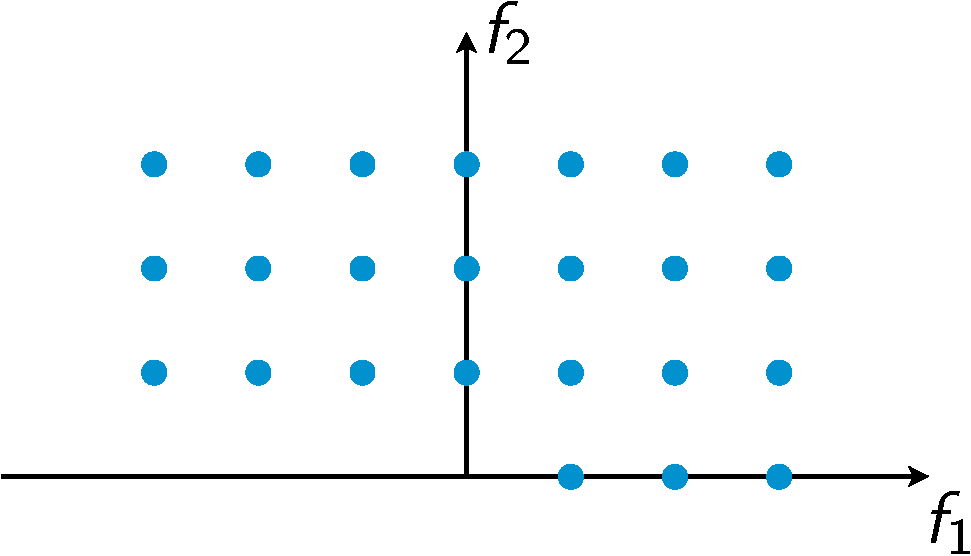
\includegraphics[width=.25\textwidth]{truncation_square.pdf}}
  \subfigure[diamond grid]{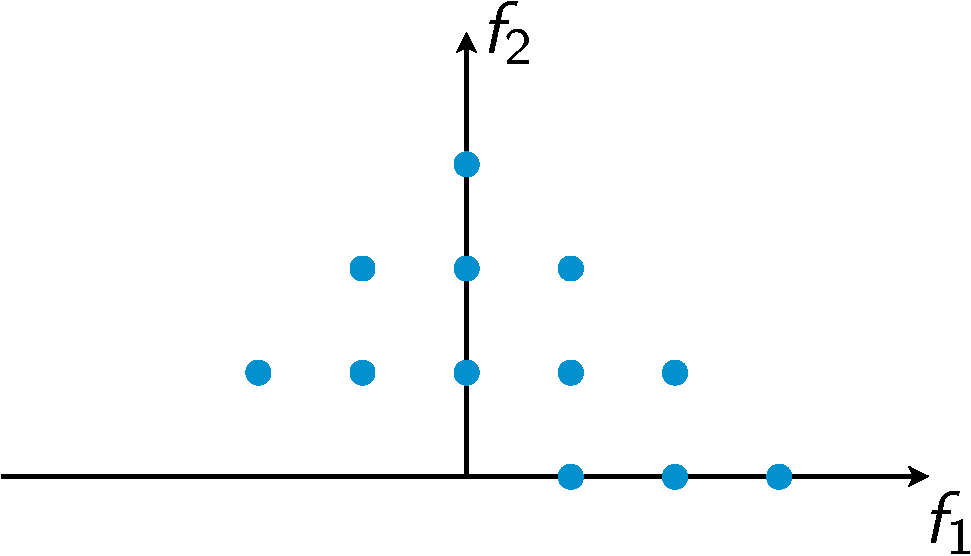
\includegraphics[width=.25\textwidth]{truncation_diamond.pdf}}
  \subfigure[cross grid]{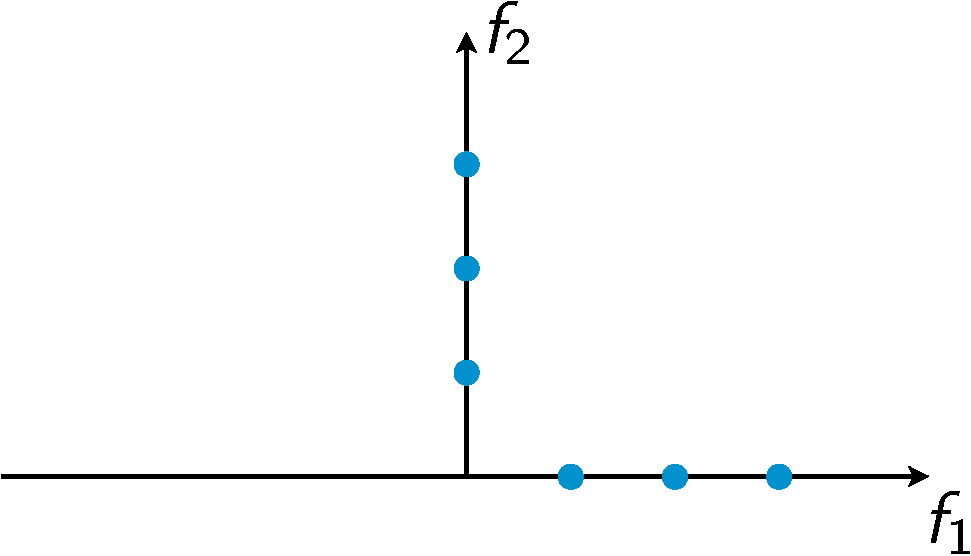
\includegraphics[width=.25\textwidth]{truncation_cross.pdf}}
  \caption{Truncation grids for reducing the set of frequencies of multi-frequential
  harmonic balance computations.}
  \label{fig:dream_hb_truncation}
\end{figure}
In the turbomachinery literature, \citet{Gopinath2007} follows the
diamond grid pattern while \citet{Ekici2007} seems to choose a
square grid pattern. In his PhD thesis, \citet{ThesisGuedeney}
first choose the frequencies by knowing which one emerge based on
a reference classical time-marching computation. Of course,
this approach can only be done \emph{a posteriori} which limits
the predictability of the method. He
also made computations with a "cross grid" truncation 
(shown in Fig.~\ref{fig:dream_hb_truncation}), this new type 
of truncation scheme only considers the harmonics of the
base frequencies. \citet{ThesisGuedeney} showed that this
truncation pattern gives
similar if not better results that the
"diamond grid" truncation pattern.  This "cross grid"
truncation pattern will be used in the current work
when using the multi-frequential approach.

\paragraph{Aeroelastic simulations}

\citet{Thomas2002a} used the method to
determine the Limit-Cycle Oscillation (LCO) solution
of a transonic airfoil configuration using the
Euler equations and \citet{Thomas2004b} extended
it to the viscous Navier-Stokes equations.
For external-flow aeroelasticity, the HB approach has 
been thoroughly 
validated by \citet{Gopinath2005, JSicot2008, Woodgate2009, JDufour2009}, 
mostly for the AGARD test cases of \citet{Davis1982}. 
\citet{JDufour2009} highlight the benefits of using a 
non-linear approach for oscillating-flap simulations
compared to linearized approaches. A one-harmonic HB simulation
gives results comparable to an expensive time-marching simulation.
\citet{Huang2013} applied the mono-frequential
HB method to the flutter prediction of the 
$11\textsuperscript{th}$ 
standard configuration for aeroelasticity~\cite{Fransson1999}.
They show that with only one harmonic, the local
harmonic response of the fluid is superimposed
with the results of a time-marching simulation.
The same study has been performed in this work
as detailed in Chap.~\ref{cha:stcf11}
and the same conclusions are drawn. These results have been
published as \citet{JSicot2012}.
In the context of the current thesis,
\citet{JSicot2013} applied the multi-frequential method to the
aeroelasticity of a contra-rotating fan, proving
the maturity of the method.


\paragraph{Transient problems}
\citet{Mavriplis2012} extended the method to 
an hybrid polynomial-harmonic balance approaches. 
It allows to use the method for maneuver simulations, 
where a part of the simulation exhibits a physical transient.
The method is also extended to overlapping mesh grids.

% \paragraph{Time sampling in the case of multi-frequential formulation}
% \citet{Gopinath2007} and \citet{Ekici2007}
% applied the multi-frequential method to
% a two-dimensional multistage compressor called
% configuration D. \citet{Ekici2007} use
% $3N+1$ evenly spaced 
% time instances to improve the condition number
% of the source term while \citet{Gopinath2007}
% stays with $2N+1$ evenly spaced time instances.
% \citet{Ekici2008a} applied the multi-frequential method
% to the effect of wake passing on the vibration of
% a turbine blade and uses $2N+1$ evenly spaced
% time instances are considered.
% \citet{JGuedeney2013} introduce non-uniform 
% time instances to minimize the condition number of multi-frequential
% computations. 
% The effect of the condition number on the stability
% of the computations is assessed along with algorithms
% to optimize the choice of the time instances.
% This allows to drastically reduce the condition number for
% any combination of frequencies, 
% while keeping only $2N+1$ samples.
% The method is then applied
% to a $1.5$ stage subsonic compressor.
% Note that a part of this work has been done in this
% thesis and will be detailed later on.

\paragraph{Gradient-based method to determine the frequency}
With the same approach as \citet{McMullen2002}, \citet{Gopinath2006}
developed a gradient-based method to estimate the frequency of a 
vortex shedding behind a cylinder and a NACA0012 airfoil 
at high angle of attack using the harmonic balance approach.
The results are superimposed with a classical time-marching approach ones.

\paragraph{Optimum shape design}
\citet{Thomas2005b} used an automatic 
differentiation compiler to derive an adjoint code
from their harmonic balance code. This adjoint code is then
evaluated on the NLR~7301 supercritical airfoil section.
The computation of the sensibilities is finally
classically compared to a finite-difference and shows
to be in good agreement with these, validating
the given approach.

\paragraph{Adaptive method}
\citet{Maple2004} presented an adaptive harmonic
balance approach. The number of harmonics is increased
if the energy of the last harmonic divided by the cumulative
sum of the energy of each harmonic is larger than a 
given threshold. During the first iterations, only
a low number of harmonic is kept. Then, when the flow
is almost converged, the adaptive harmonic balance
approach is used. This ensures that higher order harmonics
are not injected at the first iterations, when the
flow is not physical. A $86\%$ reduction in time (and
in memory footprint) is seen compared to a resolved (converged in
terms of harmonics $N$) harmonic
balance computation. This has to be compared to
the $2$ factor speed-up observed by \citet{Mosahebi2013}
with an adaptive NLFD approach.

\subsection{Numerical cost}
\label{sec:sm_hb_cost}
As mentioned before, the cost of the method is linked to
the number of simulated time instances.
In fact, each new time instance corresponds to an additional steady computation.
Thus, if \mbox{$2N+1$} time instances are considered and if $\mathdollar_{\text{RANS}}$ 
denotes the CPU and memory cost of
one steady computation, the cost of the HB method can be 
approximated by:
\begin{equation}
	\mathdollar_{\text{HB}} = (2N+1) \times \mathdollar_{\text{RANS}}.
\end{equation}
Note that \citet{Ekici2007,Ekici2008a} use $3N+1$
time instances or more to solve the bad conditioning of the
source term when using the multi-frequential formulation. 
This will be detailed later on this thesis in 
Chapter~\ref{cha:limitations_condition_number} and an innovative solution
will be proposed. In that
case, the cost is bigger and scales with the chosen number
of time instances.
